\documentclass[../main/git_course_main.tex]{subfiles}
\begin{document}

\setcounter{chapter}{2}
\chapter{Investigating your history}

\section{Overview}

In this chapter, we will:

\begin{itemize}
	\item Investigate the history using the commands \verb$git log$ and \verb$git checkout$
	\item Discuss how to compare states of the repository using \verb$git diff$
	\item Discuss regretting changes and wanting to change history
\end{itemize}

\section{Looking at the log}

To get the history of a commit, we use the command \verb$git log$. This shows all the previous commits leading to the current HEAD. It shows the following information about each commit:

% Insert information about "git log --pretty=oneline"

\begin{itemize}
	\item ID
	\item Author and the author's email
	\item Commit date
	\item Commit message
\end{itemize}

\begin{codebox}
\begin{lstlisting}
$ git log
commit 6ab77927c5dabcf7ea81bc9145ca88ebde002222
Author: Jakob Willforss <my_mail@mail.com>
Date:   Fri May 27 08:46:10 2016 +0200

    Update README

commit 7100d369d954e958632ba29dfcedf94e00f816fb
Author: Jakob Willforss <my_mail@mail.com>
Date:   Wed May 25 18:22:37 2016 +0200

    Add scripts

commit b58c6c339f8393879368db6006d0ccf738e13efa
Author: Jakob Willforss <my_mail@mail.com>
Date:   Wed May 25 18:05:36 2016 +0200

    Create README
\end{lstlisting}
\end{codebox}

%%%% GIT LOG %%%%%
\begin{figure}[h!]
\begin{bluebox}
Command: \verb$git log [--oneline]$ \\

Print the commits preceeding the current \verb$HEAD$.
\end{bluebox}
\label{command:diff}
\caption{git checkout - Check out commit or head}
\end{figure}
%%%%%%%%%%%%%%%%%%%%%%

Those commits correspond to the commits we have been creating in this chapter.
They are the three commits visualized in figure \ref{fig:third_commit_chapter3}.

\begin{figure}[h!]
	\centering
	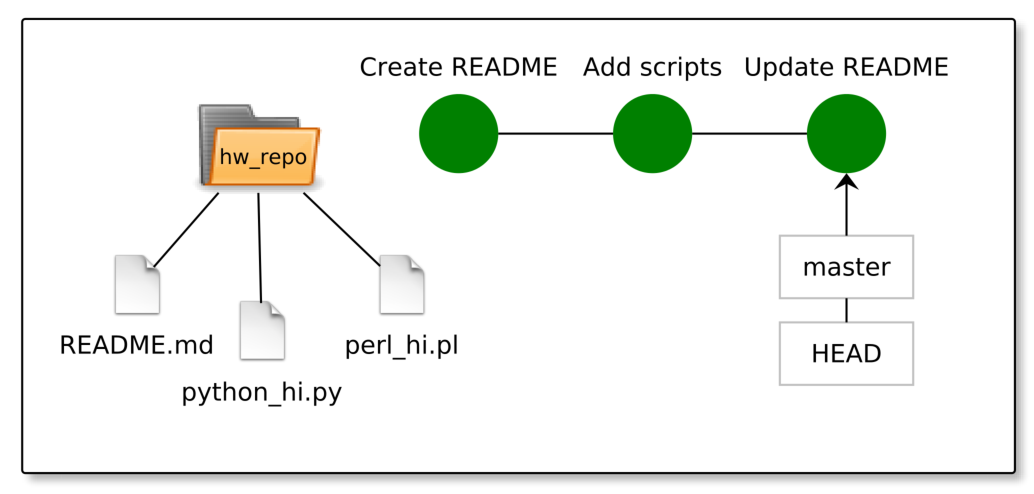
\includegraphics[width=0.8\textwidth]{../visualizations/chapter2/c26_repo_third_commit.pdf}
	\caption{The state of the file system and repository}
	\label{fig:third_commit_chapter3}
\end{figure}

Sometimes, it is useful to look at the logs in a more compact form. Then, we can add the \verb$--oneline$ flag.

\begin{codebox}
\begin{lstlisting}
$ git log --oneline
6ab7792 Update README
7100d36 Add scripts
b58c6c3 Create README
\end{lstlisting}
\end{codebox}

\begin{figure}[h!]
\begin{redbox}
When running the command \verb$git log$ you don't necessarily see all of the commits made in your repository. You get the history leading to the commit to which the \verb$HEAD$ reference currently points.
\end{redbox}
\end{figure}

\begin{figure}[h!]
\begin{redbox}
On some configurations, Git opens the \verb$git log$ output in \verb$less$. If you prefer to get it printed directly to the terminal, you can edit this setting by changing the "core-pager", the default program for visualizing longer text: \\

\verb$git config --global core.pager cat$ \\

If you later want to reset the core pager to \verb$less$, you can do so by running: \\

\verb$git config --global core.pager less$
\end{redbox}
\end{figure}

\section{Investigating differences between commits}

To compare differences between commits, we can use the command \verb$git diff$.
You can retrieve the ID for the commits using the \verb$git log$ command, and then
specify which commits you want to compare. If you only specify one commit, it will
be compared to the currently active \verb$HEAD$ commit.

\begin{codebox}
\begin{lstlisting}
$ git diff b58c6c3
... comparing HEAD to specified commit
$ git diff b58c6c3 7100d36
... comparing specified commits
\end{lstlisting}
\end{codebox}

%%%% GIT DIFF %%%%%
\begin{figure}[h!]
\begin{bluebox}
Command: \verb$git diff <commit2> [<commit2>]$ \\

Either compare current commit to target commit (one argument), or
specify two commits to compare. Prints information about what lines
that have been changed between the commits.
\end{bluebox}
\label{command:diff}
\caption{git diff - Print differences between commits}
\end{figure}
%%%%%%%%%%%%%%%%%%%%%%

\section{Going back in time}

To check out the previous commits, we can use the \verb$git checkout$ command. There are some different ways we can specify a commit:

\begin{itemize}
	\item Using the commit's ID - It is enough to specify the initial 6-8 letters
	\item Using a head pointing to the target commit
	\item A \verb$tag$ which can be used to mark important commits (more on tags in Chapter 6)
\end{itemize}

When you run the \verb$git checkout$ command, your \verb$HEAD$ is moved to the target commit and your file tree is changed to match the state represented by the commit. Make sure that you have committed your changes before running \verb$git checkout$ - otherwise, Git will protest.

Note, if you are tracing the commits your commits will have different IDs. Use them instead of the ones shown below.

\begin{codebox}
\begin{lstlisting}
$ git checkout b58c6c3  # Use your own commit ID
Note: checking out 'b58c6c3'.
... (more text)
\end{lstlisting}
\end{codebox}

The file tree is now changed to its state before adding the Hello World scripts and before adding a second line to the \verb$README.md$ We can freely investigate the current state of the file tree.

\begin{codebox}
\begin{lstlisting}
$ ls
README.md
$ cat README.md
A Hello World collection
\end{lstlisting}
\end{codebox}

\begin{figure}[h!]
\begin{redbox}
After checking out a commit, you will get a warning that you now are in a 'detached HEAD' state, meaning that your HEAD currently isn't referring to the head of a branch.
You can make commits here, but to save them you will need to create a new branch for them - otherwise
they will be removed on the next \verb$git checkout$.
\end{redbox}
\end{figure}

The state of the repository after checking out the first commit is shown in Figure \ref{fig:checkout}.

\begin{figure}[h]
	\centering
	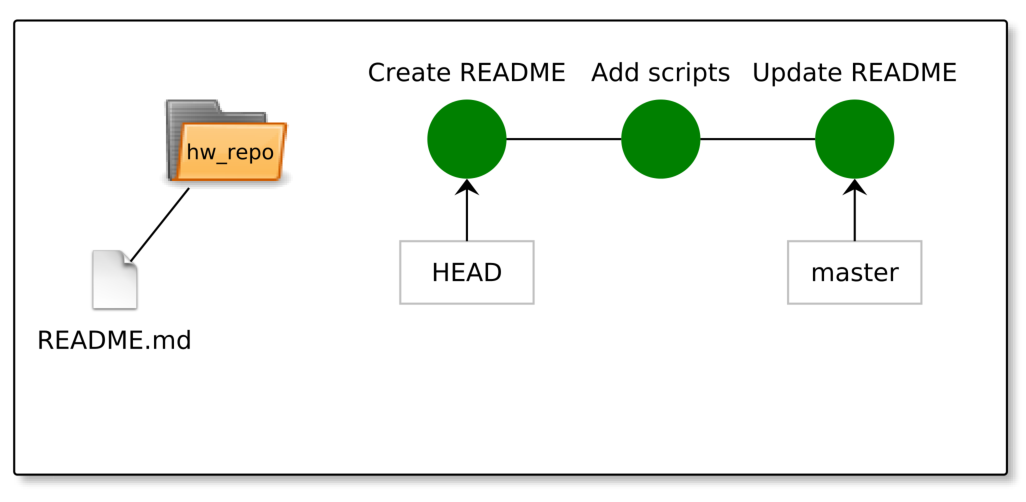
\includegraphics[width=0.8\textwidth]{../visualizations/chapter3/c31_repo_checkout_commit.pdf}
	\caption{The state of the file system and repo after checking out the first commit}
	\label{fig:checkout}
\end{figure}

How do you think the history looks now? Let's find out.

\begin{codebox}
\begin{lstlisting}
$ git log --oneline
b58c6c3 Create README
\end{lstlisting}
\end{codebox}

Now we only have one commit in the history. The reason for this is that the starting point
for the \verb$git log$ command is the first commit (\verb$b58c6c3$). That commit has no way
of seeing downstream commits as the commits only know about their parents. When going back to the master, we will see the three commits again.

We can at any time return to the master branch, and its latest commit.

\begin{codebox}
\begin{lstlisting}
$ git checkout master
Previous HEAD position was b58c6c3... Create README
Switched to branch 'master'
\end{lstlisting}
\end{codebox}

Now, the file tree is back to how we left it after the last commit. The state of the repository is shown in figure \ref{fig:back_to_master}, identical to how it was before checking out the history.

\begin{codebox}
\begin{lstlisting}
$ ls
perl_hi.pl  python_hi.py  README.md
$ cat README.md
A Hello World collection
Hello World in different languages
\end{lstlisting}
\end{codebox}

\begin{figure}[h!]
	\centering
	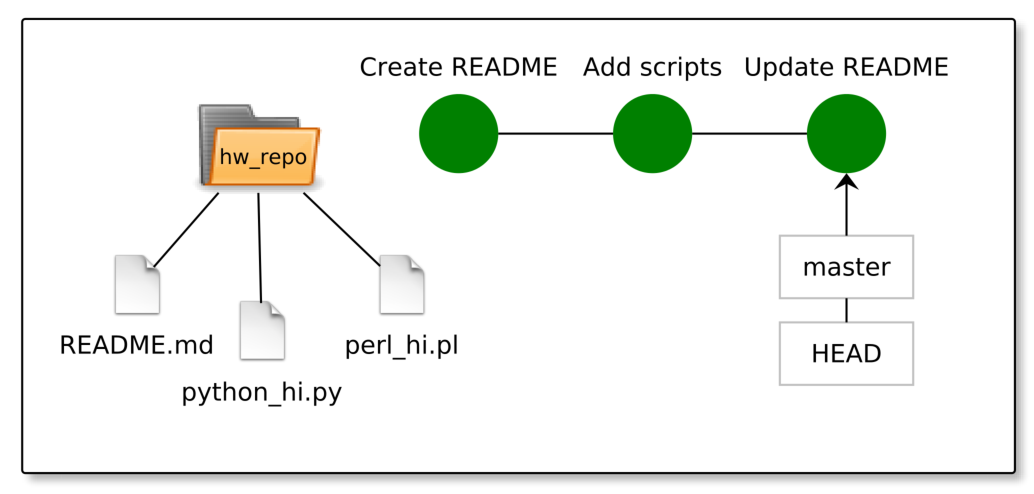
\includegraphics[width=0.8\textwidth]{../visualizations/chapter2/c26_repo_third_commit.pdf}
	\caption{The state of the repository after returning to the master}
	\label{fig:back_to_master}
\end{figure}

%%%% GIT CHECKOUT %%%%%
\begin{figure}[h!]
\begin{bluebox}
Command: \verb$git checkout <commit/head/tag>$ \\

Moves the HEAD (and changes the file tree) to target commit, branch and/or tag.
\end{bluebox}
\label{command:diff}
\caption{git checkout - Check out commit or head}
\end{figure}
%%%%%%%%%%%%%%%%%%%%%%

\section{Unstaging changes}

If we have staged the file, but realize that we don't want to include it in the next commit, we can unstage it using the command \verb$git reset$. 

\begin{codebox}
\begin{lstlisting}
$ echo '#!/usr/bin/beef' > hi.bf
$ echo '++++++++++[>+++++++>++++++++++>+++>+<<<<-]\
>++.>+.+++++++..+++.>++.<<+++++++++++++++.\
>.+++.------.--------.>+.>.' >> hi.bf
$ git add hi.bf
\end{lstlisting}
\end{codebox}

At this point, the Hello World script \verb$hi.bf$ has been created and staged, ready to be committed. If we at this point change our mind, we can unstage and remove the file from the repository.

\begin{codebox}
\begin{lstlisting}
$ git reset hi.bf  # Unstage hi.bf
$ rm hi.bf         # No traces left of hi.bf
\end{lstlisting}
\end{codebox}

Plus points if you can figure out which programming language this version
of "Hello world!" was written in.

%%%% GIT RESET %%%%%
\begin{figure}[h!]
\begin{bluebox}
Command: \verb$git reset <filepath>$ \\

Unstages a staged file.
\end{bluebox}
\label{command:reset}
\caption{git reset - Unstages a staged file}
\end{figure}
%%%%%%%%%%%%%%%%%%%%%%

\section{Reverting to older version}

If you want to reset the file to the state of an older commit, you can use the \verb$git checkout$ command instead. To demonstrate, let's do an unwanted edit to one of our scripts.

\begin{codebox}
\begin{lstlisting}
$ echo 'print("Unwanted text")' >> python_hi.py
$ git add python_hi.py
$ git commit -m "Add unwanted line"
[unwanted_edit 80d3304] Add unwanted line
 1 file changed, 1 insertion(+)
\end{lstlisting}
\end{codebox}

If we want to revert the file to a previous stage, we find the commit we want to revert it to, and check out that particular file. Then we commit the older version of the file.

\begin{codebox}
\begin{lstlisting}
$ git log --oneline
80d3304 Add unwanted line
6ab7792 Update README
7100d36 Add scripts
b58c6c3 Create README
$ cat python_hi.py
#!/usr/bin/python3
print("Hello world")
print("Unwanted text")
$ git checkout 6ab7792 python_hi.py
$ cat python_hi.py
#!/usr/bin/python3
print("Hello world")
$ git commit -m "Restore script"
[unwanted_edit 4d1a062] Restore script
 1 file changed, 1 deletion(-)
\end{lstlisting}
\end{codebox}

Note what happens if we run \verb$git log$ now. We have reverted the file \textit{by adding another commit reverting the file}.

\begin{codebox}
\begin{lstlisting}
$ git log --oneline
4d1a062 Restore script
80d3304 Add unwanted line
6ab7792 Update README
7100d36 Add scripts
b58c6c3 Create README
\end{lstlisting}
\end{codebox}

\begin{figure}[h!]
	\centering
	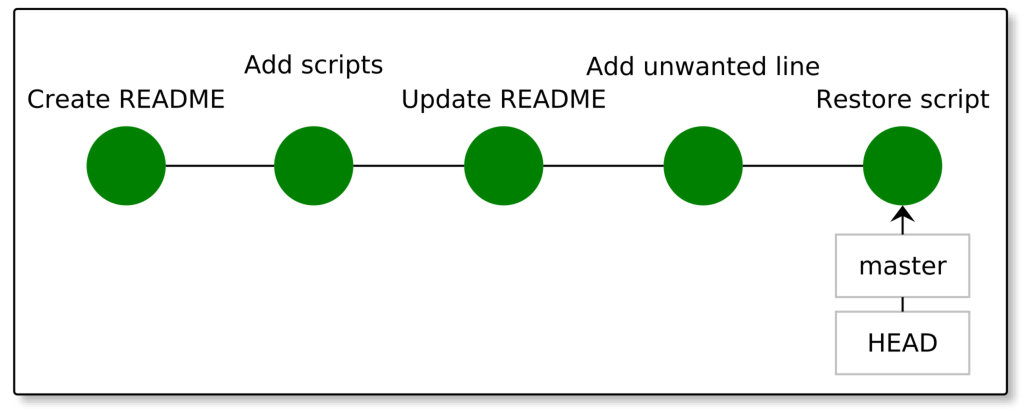
\includegraphics[width=0.8\textwidth]{../visualizations/chapter3/c32_fixed_unwanted_changes.pdf}
	\caption{Repository after correcting unwanted edits in fourth commit}
	\label{fig:correcting_unwanted_changes}
\end{figure}

This means that the version of the file where it had an extra line still exists within the Git history. This is good - History is history. We can write new history which changes a file back to an earlier state, but should almost, almost never fiddle with the existing history. The repository for the final state is shown in figure \ref{fig:correcting_unwanted_changes}. Note that the state of the \textit{file tree} would be exactly the same if the third commit were checked out.

\section{Thoughts on regretting commits}

It is generally considered bad practice to go back and edit existing commits (instead of creating new commits reverting their changes), \textit{especially} if you have pushed them to a remote - sent them to a central repository which you share with others.
If you start editing the history on a collaborative project, you not only change the history for yourself but for your collaborators too.

Under exceptional circumstances, it might be reasonable to fiddle with the history. For example if you accidentally commit 20 GB of sequence data
to your repository, it might be better to remove the commit than sending it to your collaborators. Otherwise, it is generally better
to create another commit which undoes your mistakes.

\newpage
\section{Exercises}

\subsection{Trying out the commands}

Let's continue working with the repository that you created in the exercises for Chapter 2.

\begin{enumerate}
	\item Print the log of your repository. Try both full format and one-line format. Can you easily trace the history of your files based on your commit messages?
	\item Take a look at your current file tree (simply by using \verb$ls$ and \verb$cat$). Run \verb$git checkout$ for one of your commits. Check the file system again. Can you see the changes?
	\item Before going back to the master, compare the \verb$git log$ output to what you got before. Do you see a difference? Why?
	\item Go back to the \verb$master$.
	\item Revert one of your files to an older version and commit the revert.
	\item Navigate around in your repository until you feel comfortable using the commands \verb$git log$ and \verb$git checkout$.
\end{enumerate}

\subsection{Understanding "git checkout" and HEAD}

\begin{enumerate}
	\item For the previous exercises, visualize how each step affects the file tree, the repository and in particular the HEAD.
\end{enumerate}

\subsection{Exploring .git (*)}

\begin{enumerate}
	\item Take a look into the .git-directory located at the top level in your Git repository. This directory contains everything related to the repository.
	\item See if you can figure out how files in this directory are related to the output you get from for example running \verb$git log$.
\end{enumerate}

\newpage
\section{Recap}

\subsection{Concepts}

\begin{itemize}
	\item How are the file tree and the HEAD affected when running \verb$git checkout$? Is the repository affected?
	\item How are the output from \verb$git log$ and the \verb$HEAD$ related?
	\item How do you best handle resetting a particular file to a previous version?
\end{itemize}

\subsection{Commands}

\begin{itemize}
	\item \verb$git log [--oneline]$
	\item \verb$git checkout <commit ID/head/tag>$
\end{itemize}

\end{document}
